\definecolor{codegreen}{rgb}{0,0.6,0}
\definecolor{codegray}{rgb}{0.5,0.5,0.5}
\definecolor{codepurple}{rgb}{0.58,0,0.82}
\definecolor{backcolour}{rgb}{0.95,0.95,0.92}

\lstdefinestyle{mystyle}{
	backgroundcolor=\color{backcolour},   
	commentstyle=\color{codegreen},
	keywordstyle=\color{magenta},
	numberstyle=\tiny\color{codegray},
	stringstyle=\color{codepurple},
	basicstyle=\ttfamily\footnotesize,
	breakatwhitespace=false,         
	breaklines=true,                 
	captionpos=b,                    
	keepspaces=true,                 
	numbers=left,                    
	numbersep=5pt,                  
	showspaces=false,                
	showstringspaces=false,
	showtabs=false,                  
	tabsize=2
}

\lstset{style=mystyle}


\chapter{Prediktivni modeli primjenom strojnog učenja}

Kako bismo bolje razumjeli što film čini uspješnim ili neuspješnim, provele smo analizu dobivenog skupa podataka primjenom strojnog učenja. Cilj nam je bio razviti model koji može čim točnije predviđati uspjeh filma na temelju njegovih karakteristika.
\\
\section{Priprema podataka}
Iz dobivenih podataka izbacile smo retke kojima su nedostajali neki podaci. Takvih je redaka bilo 1261. Također, uklonile smo stupce koji su sadržavali jedinstvene ili skoro jedinstvene vrijednosti (\textit{movie\_title, movie\_imdb\_link, plot\_keywords, genres}). Još smo izbacile tekstualne stupce koji su bili prekorelirani s nekim numeričkim stupcem. Na primjer, \textit{actor\_1\_name} je prekoreliran s \textit{actor\_1\_facebook\_likes}. 

\lstinputlisting[language=R]{../R/001.R} 
Preostale nenumeričke stupce pretvorile smo u tip integer. 

\lstinputlisting[language=R]{../R/002.R}

Značajka koju predviđamo je \textit{imdb\_score}. To broj zaokružen na jednu decimalu, pa smo za bolje rezultate uspjeh filma podijelile u tri skupine: loš, osrednji i dobar, a stupac imdb\_score smo zbog prekoreliranosti uklonile. 

\lstinputlisting[language=R]{../R/003.R}

Graf \ref{fig:ml1} prikazuje omjer broja filmova po uspjehu. Filmova koji su ocijenjeni kao loši znatno je manje od ostalih. Točnije, loših je filmova 43, osrednjih 1981, a dobrih 1746.

\begin{figure}
	\centering
	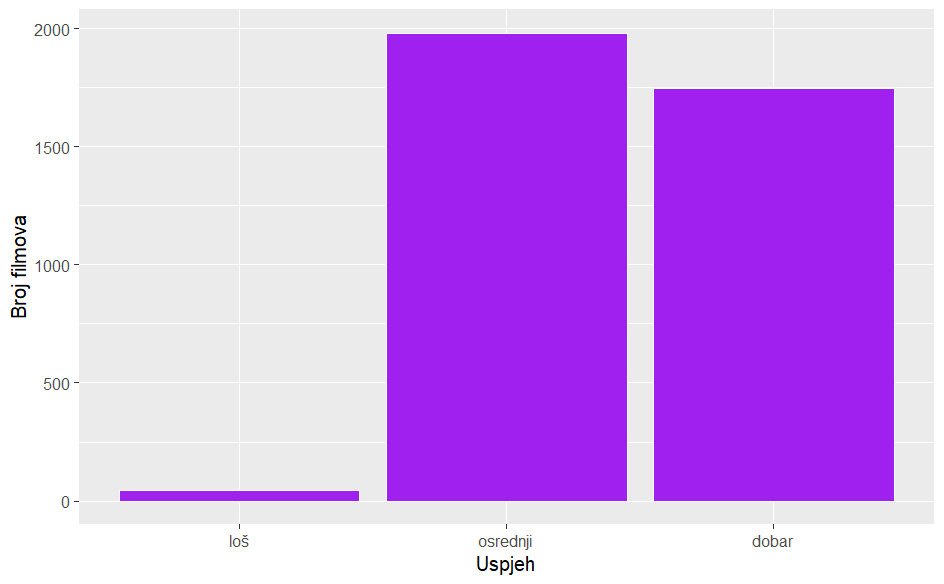
\includegraphics[width=15cm]{../figures/expl/001.png}
	\caption{Podjela filmova po uspjehu}
	\label{fig:ml1}
\end{figure}


\lstinputlisting[language=R]{../R/004.R}

\begin{center}
	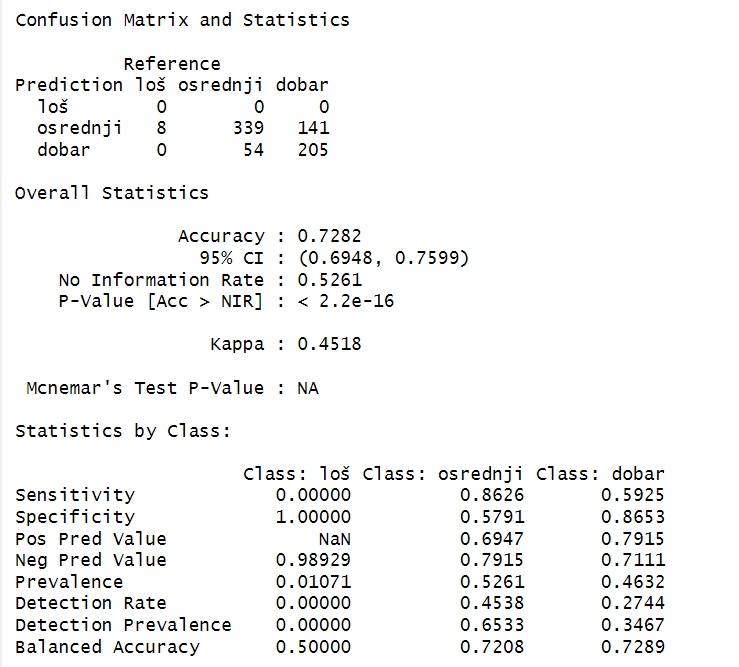
\includegraphics{../figures/expl/002.png}
\end{center}

\lstinputlisting[language=R]{../R/005.R}

\begin{center}
	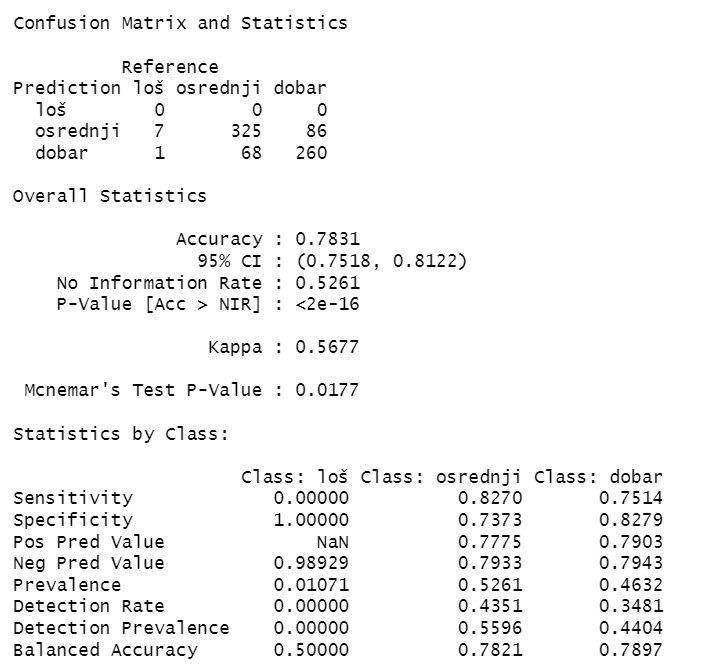
\includegraphics{../figures/expl/003.png}
\end{center}

\lstinputlisting[language=R]{../R/006.R}

\begin{center}
	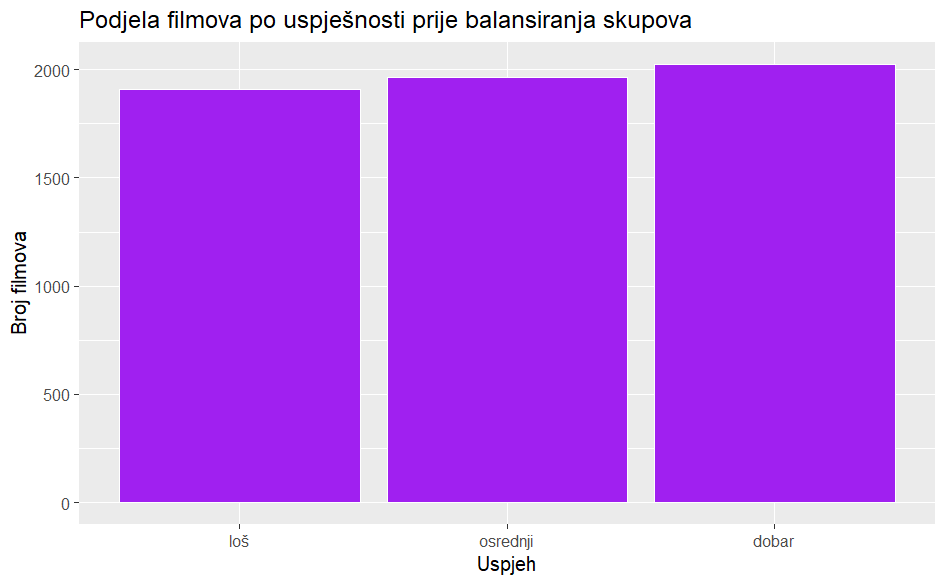
\includegraphics[width=15cm]{../figures/expl/004.png}
\end{center}

\begin{center}
	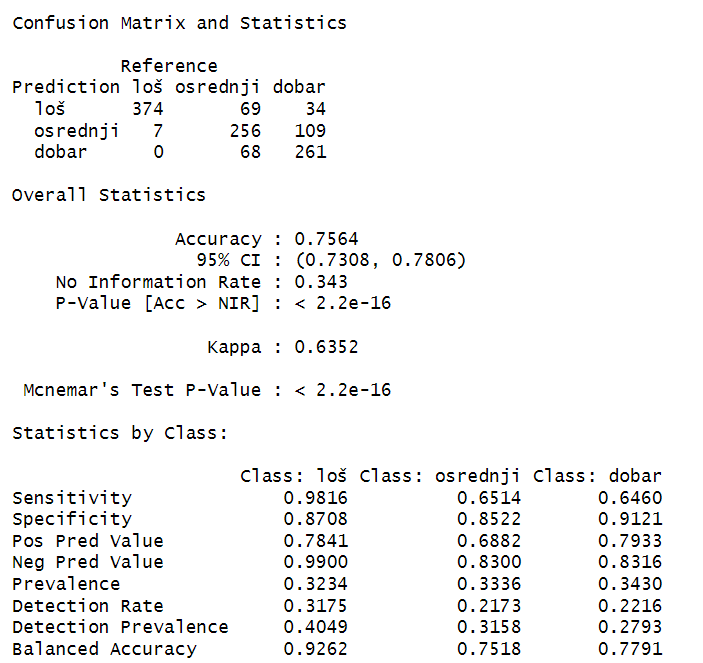
\includegraphics{../figures/expl/005.png}
\end{center}

\begin{center}
	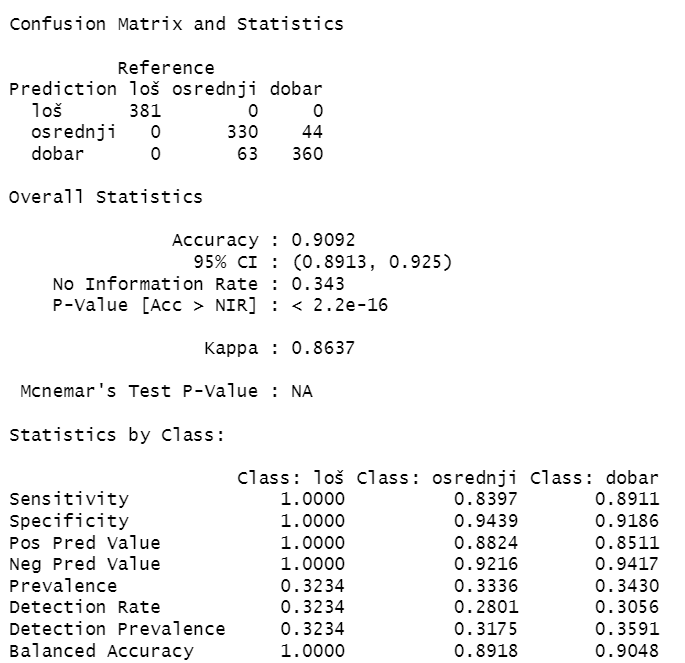
\includegraphics{../figures/expl/006.png}
\end{center}

\begin{center}
	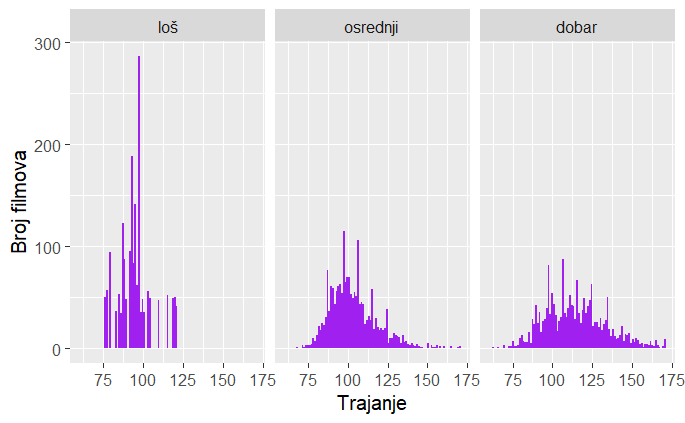
\includegraphics[width=15cm]{../figures/expl/007.png}
\end{center}

\begin{center}
	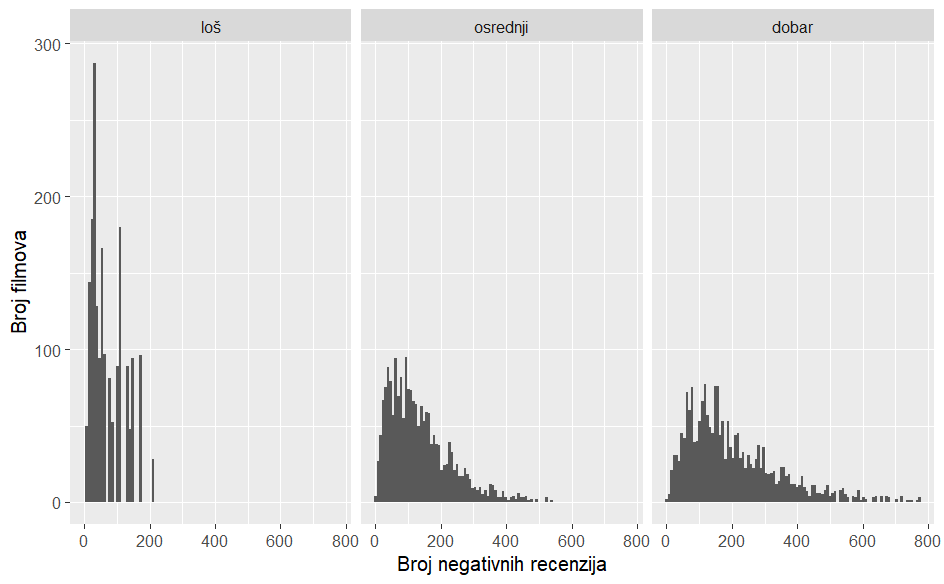
\includegraphics[width=15cm]{../figures/expl/008.png}
\end{center}


\eject